% LaTeX figure snippets. The writing agent will embed these inline in main.tex.

\begin{figure}[t]
  \centering
  \begin{subfigure}{0.48\linewidth}
    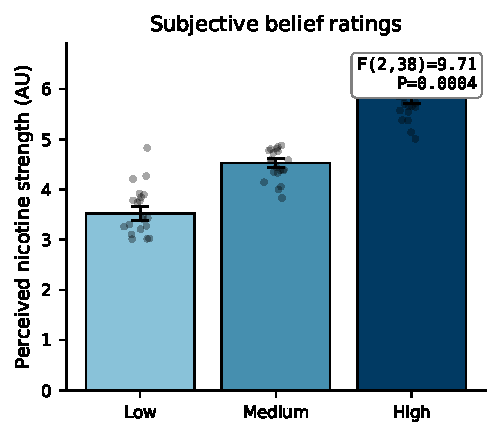
\includegraphics[width=\linewidth]{figures/fig1b_belief_ratings.pdf}
    \caption{}
    \label{fig:belief-ratings}
  \end{subfigure}\hfill
  \begin{subfigure}{0.48\linewidth}
    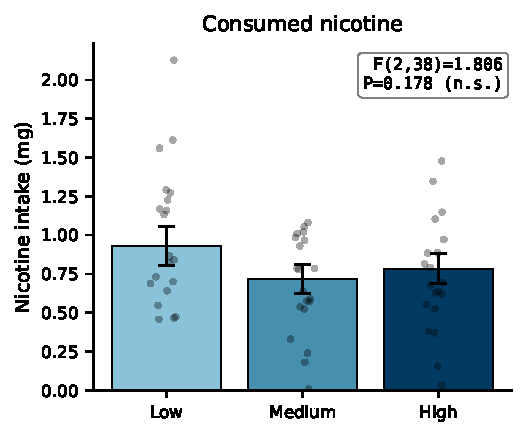
\includegraphics[width=\linewidth]{figures/fig1c_nicotine_intake.pdf}
    \caption{}
    \label{fig:nicotine-intake}
  \end{subfigure}
  \caption{\textbf{Belief manipulation and sanity checks.} (\subref{fig:belief-ratings}) Subjective perceived nicotine strength scales with the instructed label (low $3.52 \pm 0.61$, medium $4.52 \pm 0.41$, high $5.82 \pm 0.47$ AU; rmANOVA $F(2,38)=9.71$, $P=0.0004$, partial $\eta^2=0.34$). (\subref{fig:nicotine-intake}) Consumed nicotine does not differ across belief conditions (low $0.928 \pm 0.56$, medium $0.719 \pm 0.423$, high $0.783 \pm 0.434$ mg; $F(2,38)=1.806$, $P=0.178$). Cotinine and exhaled carbon monoxide are similarly invariant across conditions ($P=0.393$ and $P=0.698$; not shown). Bars, group means; points, participants; error bars, SEM.}
  \label{fig:fig1}
\end{figure}

\begin{figure}[t]
  \centering
  \begin{subfigure}{0.49\linewidth}
    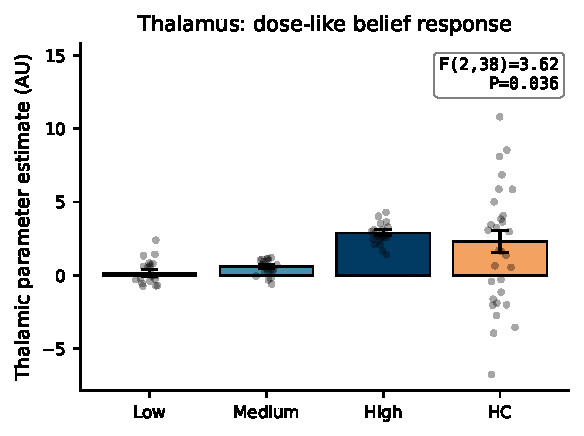
\includegraphics[width=\linewidth]{figures/fig2b_thalamus_bars.pdf}
    \caption{}
    \label{fig:thalamus-bars}
  \end{subfigure}\hfill
  \begin{subfigure}{0.49\linewidth}
    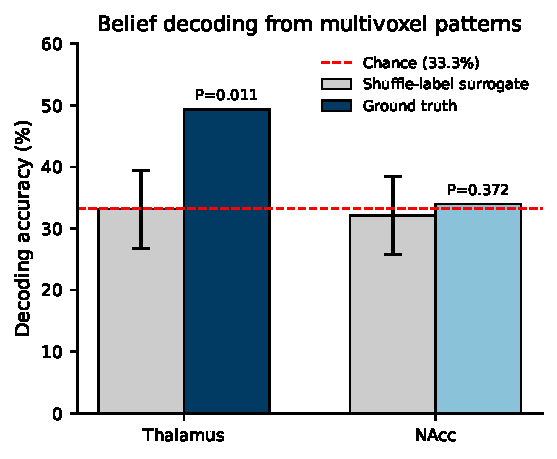
\includegraphics[width=\linewidth]{figures/fig2d_decoding.pdf}
    \caption{}
    \label{fig:decoding}
  \end{subfigure}
  \caption{\textbf{Thalamic activity encodes a dose-like belief signal.} (\subref{fig:thalamus-bars}) Value-tracking parameter estimates in an independent thalamic ROI scale parametrically with instructed belief (low $0.157 \pm 1.047$, medium $0.601 \pm 0.714$, high $2.914 \pm 0.865$ AU; rmANOVA $F(2,38)=3.62$, $P=0.036$, partial $\eta^2=0.16$). Non-smoking healthy controls (HC, $n=31$, $2.318 \pm 4.258$ AU) do not differ significantly from any single smoker condition (two-sample $t$-tests, all $P>0.05$). (\subref{fig:decoding}) Multivoxel decoding of belief condition from thalamic patterns reaches 49.3\% (chance 33.3\%, shuffle-label surrogate $33.1 \pm 6.3$\%, $P=0.011$), whereas decoding from nucleus accumbens patterns is at 34.0\% (surrogate $32.1 \pm 6.3$\%, $P=0.372$). Bars, means; error bars, SEM or shuffle surrogate SD.}
  \label{fig:fig2}
\end{figure}

\begin{figure}[t]
  \centering
  \begin{subfigure}{0.49\linewidth}
    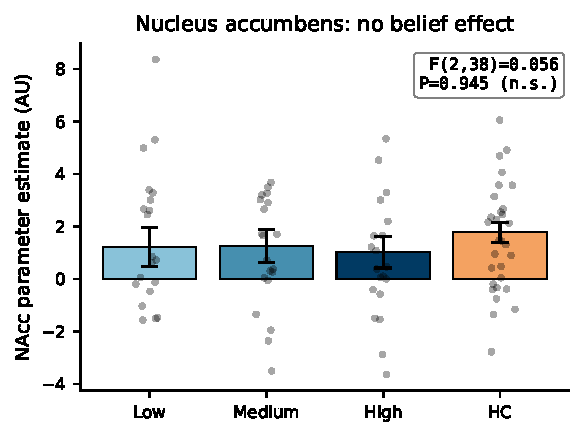
\includegraphics[width=\linewidth]{figures/fig3b_nacc_bars.pdf}
    \caption{}
    \label{fig:nacc-bars}
  \end{subfigure}\hfill
  \begin{subfigure}{0.49\linewidth}
    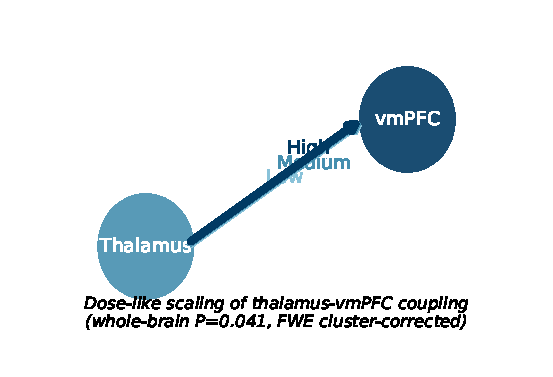
\includegraphics[width=\linewidth]{figures/fig4_ppi_schematic.pdf}
    \caption{}
    \label{fig:ppi-schematic}
  \end{subfigure}
  \caption{\textbf{Negative striatal result and thalamus-vmPFC coupling.} (\subref{fig:nacc-bars}) Nucleus accumbens parameter estimates do not differentiate belief conditions (smokers low $1.228 \pm 3.329$, medium $1.248 \pm 2.828$, high $1.016 \pm 2.6983$ AU; rmANOVA $F(2,38)=0.056$, $P=0.945$) and are comparable to HC ($1.781 \pm 2.138$ AU; all between-group $t$-tests $P>0.25$). Putamen and caudate also show no belief effect ($P=0.327$ and $P=0.781$). (\subref{fig:ppi-schematic}) Schematic of the key psychophysiological-interaction finding: functional coupling between the thalamus and vmPFC scales with belief dose (whole-brain $P=0.041$, FWE cluster-corrected at cluster-defining $P<0.005$, $k=50$).}
  \label{fig:fig3}
\end{figure}
